\section{Experiment 2: Hydrogen}

We use three visible hydrogen lines to test the Balmer relation. The fit gives $R=1.11\times10^7\pm4\times10^5\,\text{m}^{-1}$ and $n_f=2.01\pm0.02$, consistent with the reference Rydberg constant and transitions into the $n=2$ level.

\subsection{Setup and reference measurements}

We placed the hydrogen discharge tube behind the central opening of the spectrometer scale and viewed it through the same transmission grating used for helium. The scale and grating positions were $14.35\,\text{cm}$ and $42.20\,\text{cm}$, giving $L_H=27.85\,\text{cm}$. We measured the apparent first order offsets from the central image. Distinct red, cyan, and blue to violet lines form a useful hydrogen fingerprint.

\begin{figure}[H]
\centering
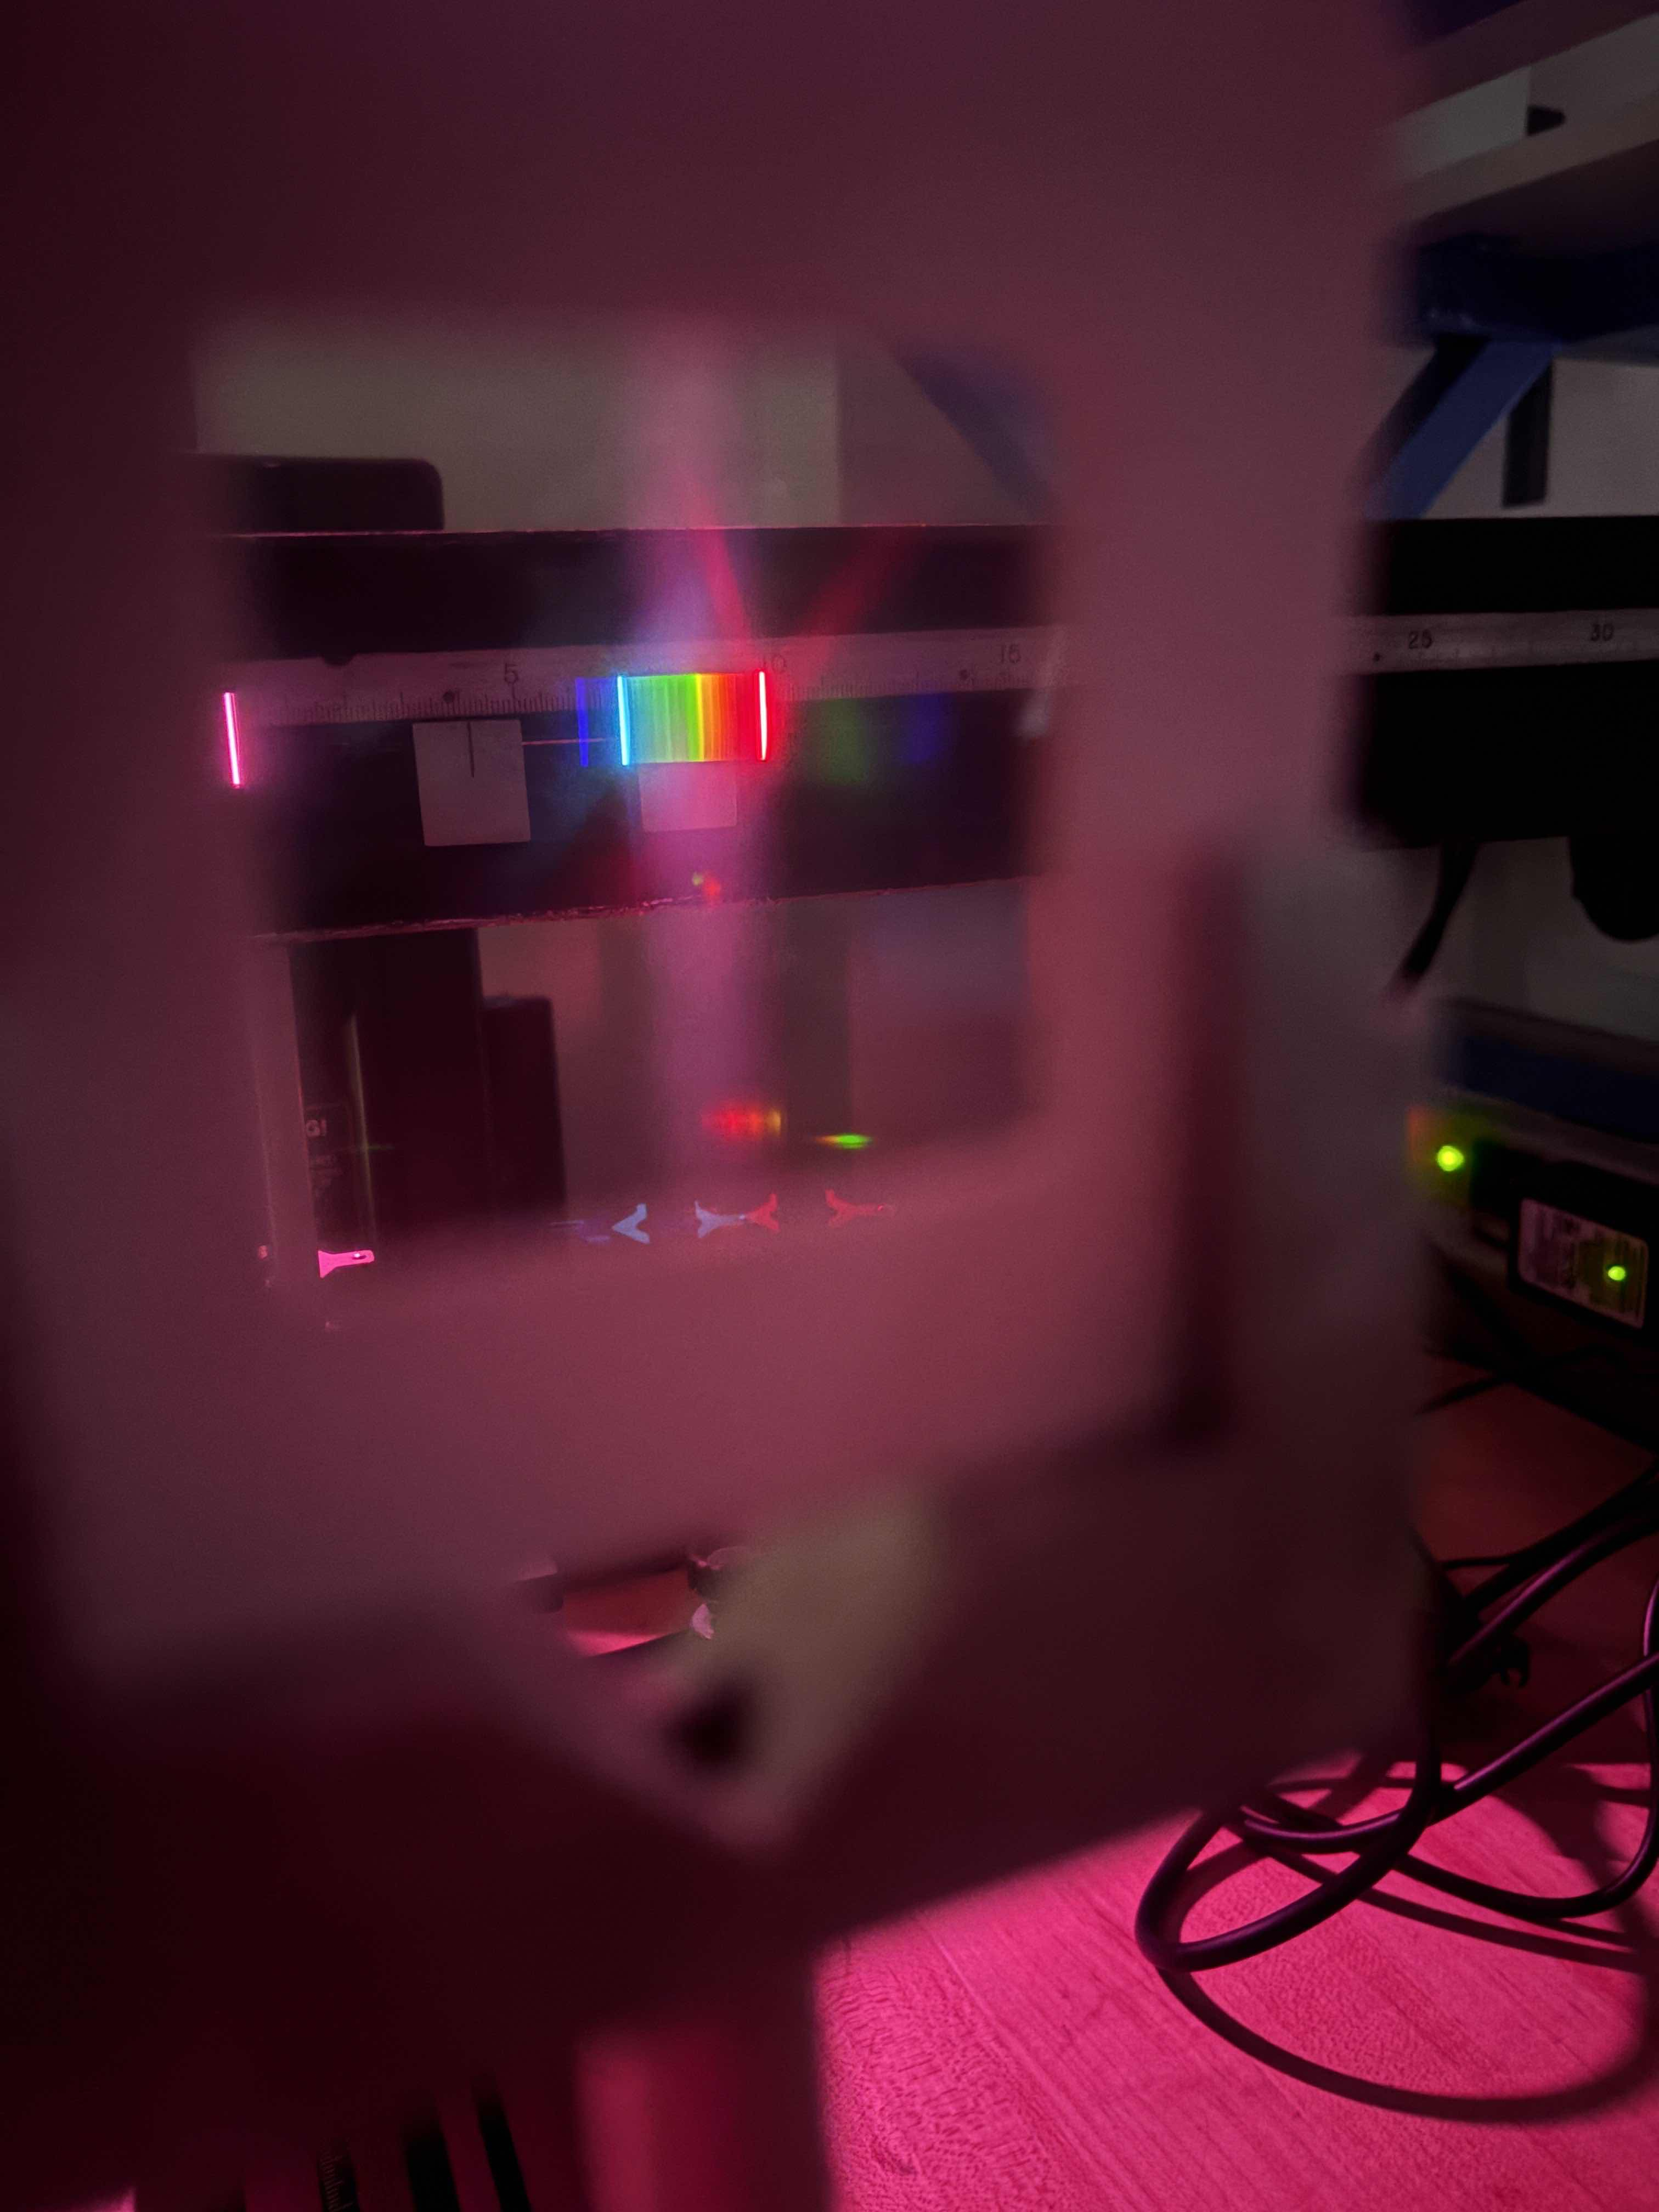
\includegraphics[width=\linewidth,trim=250bp 2432bp 1124bp 1100bp,clip]{Photos/setup2.jpg}
\caption{Hydrogen spectrum viewed through the transmission grating. The prominent lines appear against a broader background. The photograph records the observed pattern, rather than measured line intensities.}
\label{fig:hydrogen-photo}
\end{figure}

\begin{figure}[H]
\centering
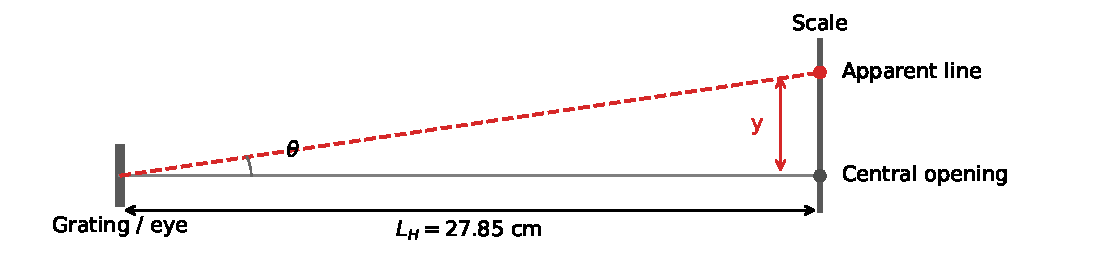
\includegraphics[width=\linewidth]{figures/hydrogen_geometry.pdf}
\caption{Geometry used to convert apparent line position to wavelength. The dashed line is a viewing construction, not a projected beam. The displacement $y$ is measured from the central opening.}
\label{fig:hydrogen-geometry}
\end{figure}

The four helium D3 placements in Experiment 1 give the position statistics
\begin{align}
\bar y_D&=\frac{1}{N}\sum_{j=1}^{N}y_j, \\
s_y^2&=\frac{1}{N-1}\sum_{j=1}^{N}(y_j-\bar y_D)^2, \\
u_D&=\frac{s_y}{\sqrt{N}}.
\end{align}
For $N=4$, we obtain $\bar y_D=11.22\pm0.05\,\text{cm}$, $s_y=0.09\,\text{cm}$, and $u_D=0.05\,\text{cm}$. Following the handout, the standard error $u_D$ describes the mean reference position, while the sample standard deviation $s_y$ describes a new line placement. We retain the unrounded values in all calculations.

\clearpage
\subsection{Wavelengths and propagated uncertainty}

For a first order maximum, the grating equation and viewing geometry give
\begin{align}
\lambda&=d\sin\theta, \\
\sin\theta&=\frac{y}{\sqrt{L^2+y^2}}.
\end{align}
The largest hydrogen angle is about $19^\circ$, so we retain the full geometry. Using $\lambda_D=587.6\,\text{nm}$ and the helium separation $L_{He}=36.58\,\text{cm}$,
\begin{align}
d&=\lambda_D\frac{\sqrt{L_{He}^2+\bar y_D^2}}{\bar y_D}=2003\pm8\,\text{nm}, \\
u_d&=\frac{\lambda_D L_{He}^2}{\bar y_D^2\sqrt{L_{He}^2+\bar y_D^2}}u_D.
\end{align}
The reference wavelength is held fixed. Bench position uncertainties were not recorded, so the quoted uncertainties also hold both separations fixed.

For a hydrogen position $y$,
\begin{align}
\lambda&=d\frac{y}{\sqrt{L_H^2+y^2}}, \\
u_\lambda^2&=\left(\frac{\lambda}{d}u_d\right)^2+
\left(\frac{dL_H^2}{(L_H^2+y^2)^{3/2}}s_y\right)^2.
\end{align}
Position placement contributes about $6\,\text{nm}$ per line, compared with about $2\,\text{nm}$ from the grating spacing. Visual placement therefore dominates the reported uncertainty. The apparent line width of about $0.1\,\text{cm}$ is comparable to the measured position scatter.

\begin{table}[H]
\centering
\begin{tabular}{ccccc}
\toprule
Line & $y$ / $\text{cm}$ & Calculated $\lambda$ / $\text{nm}$ & Predicted / $\text{nm}$ & $Z_\lambda$ \\
\midrule
Red, $3\to2$ & $9.78\pm0.09$ & $664\pm6$ & 656.1 & 1.2 \\
Cyan, $4\to2$ & $6.97\pm0.09$ & $486\pm6$ & 486.0 & 0.06 \\
Blue/violet, $5\to2$ & $6.24\pm0.09$ & $438\pm6$ & 433.9 & 0.63 \\
\bottomrule
\end{tabular}
\caption{Wavelengths and Balmer assignments. Predictions use the handout's Rydberg constant before rounding. Each $Z_\lambda$ is the measured minus predicted wavelength divided by its propagated uncertainty.}
\label{tab:hydrogen-wavelengths}
\end{table}

\begin{figure}[H]
\centering
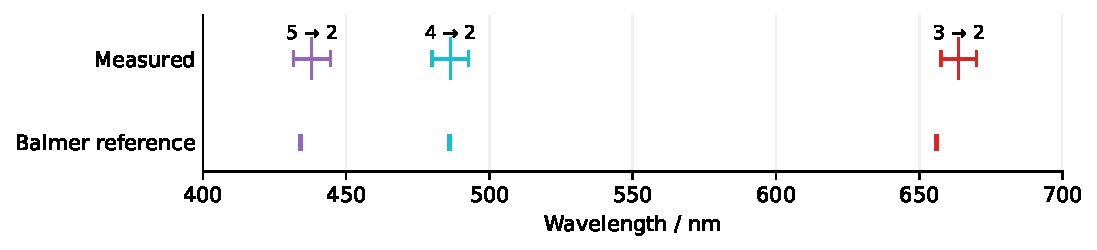
\includegraphics[width=\linewidth]{figures/hydrogen_spectrum.pdf}
\caption{Measured and predicted line positions, labeled by transition. Horizontal bars show wavelength uncertainties. Mark heights are schematic and do not represent measured brightness.}
\label{fig:hydrogen-spectrum}
\end{figure}

The red line has the largest error from the prediction, about $8\,\text{nm}$ or $1.2$ quoted uncertainties. The three lines are compatible with the first three Balmer transitions. Their wavelength ordering and separation also support these assignments. The single line checks are correlated because the same calculated grating spacing enters every wavelength.

\clearpage
\subsection{Bohr fit and statistical interpretation}

Quantized electron energy gaps give the Balmer relation. Defining $x=n_i^{-2}$ and $w=\lambda^{-1}$ makes it linear,
\begin{align}
w&=R(n_f^{-2}-x)=mx+b, \\
R&=-m, \\
n_f&=\sqrt{-\frac{m}{b}}.
\end{align}
We fit all three points with slope and intercept free. The weighted regression retains the common grating contribution to the wavelength covariance. We use $u_R=u_m$ and propagate the full slope and intercept covariance into $u_{n_f}$.

\begin{figure}[H]
\centering
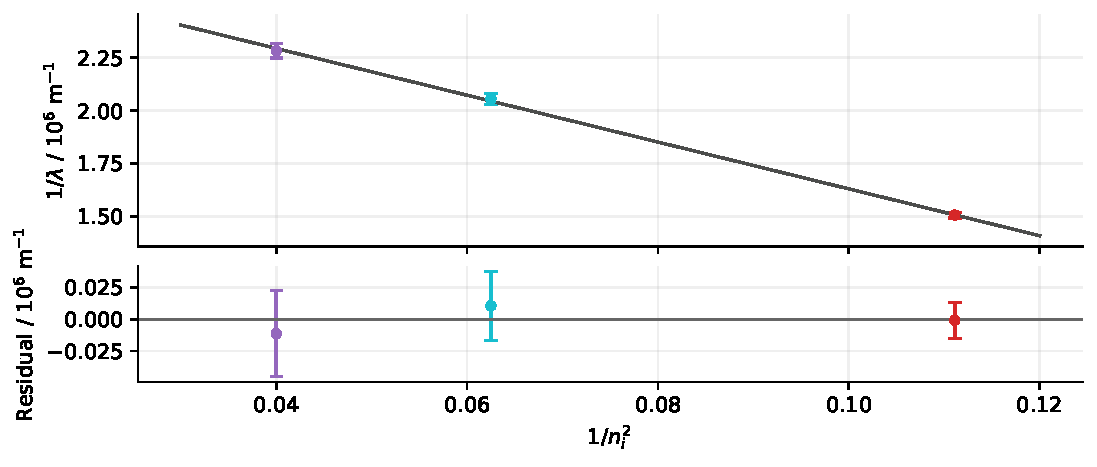
\includegraphics[width=\linewidth]{figures/hydrogen_fit.pdf}
\caption{Reciprocal wavelength fit and raw residuals $w-w_{\text{fit}}$, with the same propagated uncertainties. The quantum numbers are fixed.}
\label{fig:hydrogen-fit}
\end{figure}

\begin{table}[H]
\centering
\begin{tabular}{cccc}
\toprule
Quantity & Calculated result & Reference & Difference / uncertainty \\
\midrule
$m$ / $10^7\,\text{m}^{-1}$ & $-1.11\pm0.04$ & -- & -- \\
$b$ / $10^6\,\text{m}^{-1}$ & $2.74\pm0.04$ & -- & -- \\
$R$ / $10^7\,\text{m}^{-1}$ & $1.11\pm0.04$ & 1.09737 & 0.23 \\
$n_f$ & $2.01\pm0.02$ & 2 & 0.47 \\
\bottomrule
\end{tabular}
\caption{Fit parameters and derived values. The last two rows come from the same fit.}
\label{tab:hydrogen-fit-results}
\end{table}

For residual vector $\mathbf r$ and reciprocal wavelength covariance $C_w$, the fit statistic is
\begin{equation}
\chi^2=\mathbf r^{T}C_w^{-1}\mathbf r.
\end{equation}
The free fit has $\nu=3-2=1$ degree of freedom and $\chi^2=\chi_\nu^2=0.29$, with $p\approx0.59$. Comparing all three wavelengths with the fixed Balmer prediction gives $\chi^2=1.8$ for three degrees of freedom and $p\approx0.62$. Both checks are consistent with the model.

These approximate $p$ values treat the estimated reading errors as fixed Gaussian uncertainties. Four reference placements and one fit residual degree of freedom provide limited evidence about the error scale. We retain the input uncertainties despite the small residuals.

Alignment and unrecorded bench position uncertainty remain possible systematic errors. A common wavelength scale error changes $R$ but cancels from the slope to intercept ratio for $n_f$. Thus $n_f=2$ checks the spectral pattern more directly than the absolute scale. The results support the Balmer model at our precision. A hydrogen reflection grating trace and fluorescence wavelengths were not recorded.
